\documentclass{beamer}
\usepackage[utf8]{inputenc}
\usepackage[spanish]{babel}
\usepackage{amsmath, amsthm, amssymb}
\usepackage{enumitem}
\usepackage{graphicx,caption}
\usepackage{tikz}

\setitemize{label=\usebeamerfont*{itemize item}%
  \usebeamercolor[fg]{itemize item}
  \usebeamertemplate{itemize item}}

\usepackage[absolute,overlay]{textpos}
  \setlength{\TPHorizModule}{1cm}
  \setlength{\TPVertModule}{1cm}

\AtBeginSection[]
{
  \begin{frame}{Tabla de contenido}
    \tableofcontents[currentsection]
  \end{frame}
}
\beamertemplatenavigationsymbolsempty
\setbeamertemplate{footline}[frame number]
\setbeamertemplate{theorems}[numbered]

\newtheorem{teo}{Teorema}
\newtheorem{conj}{Conjetura}

\title{Tamaño máximo de un thrackle de triángulos}
\author [Santiago León O.] {Santiago León Ortiz\\ {\small Asesora: Dra. Dolores Lara Cuevas}}
\institute [Cinvestav, Computación] { }
\date{16 de octubre de 2017}

\usetheme{Madrid}

\setbeamertemplate{footline}
{
  \leavevmode%
  \hbox{%
  \begin{beamercolorbox}[wd=.3\paperwidth,ht=2.25ex,dp=1ex,center]{author in head/foot}%
    \usebeamerfont{author in head/foot}\insertshortauthor
  \end{beamercolorbox}%
  \begin{beamercolorbox}[wd=.4\paperwidth,ht=2.25ex,dp=1ex,center]{title in head/foot}%
    \usebeamerfont{title in head/foot}\insertshorttitle
  \end{beamercolorbox}%
  \begin{beamercolorbox}[wd=.3\paperwidth,ht=2.25ex,dp=1ex,right]{date in head/foot}%
    \usebeamerfont{date in head/foot}\insertshortdate{}\hspace*{2em}
    \insertframenumber{}\hspace*{2ex} 
  \end{beamercolorbox}}%
  \vskip0pt%
}

\begin{document}
\begin{frame}
    \parbox[c]{2cm}{\centering
      
\includegraphics[width=1.5cm]{cinvestavlogo.png}
    }
    \parbox[c]{\dimexpr\paperwidth-3cm\relax}{\centering
      {\large Departamento de Computación\\ Cinvestav Zacatenco}
    }
  \maketitle
\end{frame}

\begin{frame}
  \frametitle{Thrackles de triángulos}
  \begin{figure}[htb]
    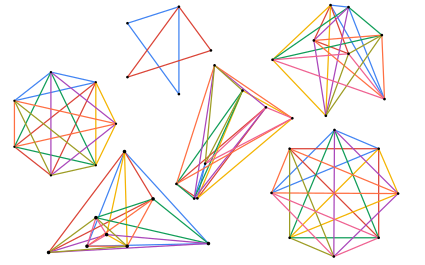
\includegraphics{examples.pdf}
  \end{figure}
\end{frame}

\begin{frame}
  \frametitle{¿Cuántos conjuntos de puntos hay?}
  Hay un número infinito de formas de elegir un sólo punto en el plano.
  \begin{figure}[htb]
    \includegraphics<1>{puntos.pdf}
    \includegraphics<2>{puntos_1.pdf}
  \end{figure}
  \begin{block}{Posición general}
    Conjuntos de puntos en los que no hay 3 en una misma
    recta.
  \end{block}
\end{frame}

\begin{frame}
  \frametitle{Tipos de orden}
  \begin{block}{}
    Son clases de equivalencia de conjuntos de puntos que comparten las mismas
    propiedades combinatorias.
  \end{block}
  \begin{figure}[htb]
    \includegraphics<1>{tipos_de_orden.pdf}
    \includegraphics<2>{tipos_de_orden_1.pdf}
  \end{figure}
\end{frame}

\begin{frame}
  \frametitle{Base de datos de tipos de orden [O. Aichholzer]}
  Hay una base de datos con conjuntos de $n$ puntos para cada tipo de orden.
  Hasta $n=10$.
  \begin{figure}[htb]
    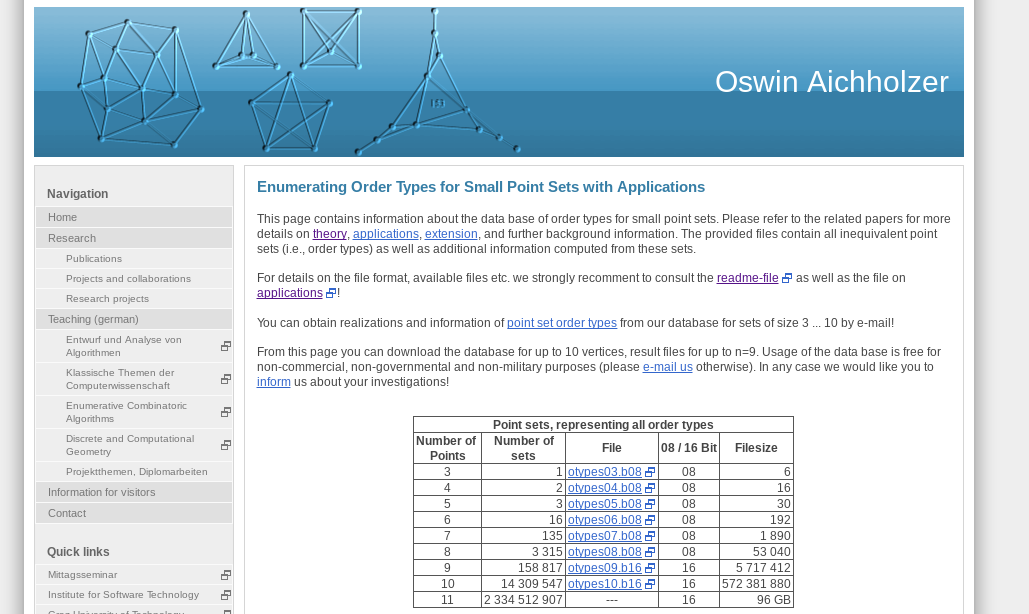
\includegraphics[width=0.8\textwidth]{base_de_datos.png}
  \end{figure}
\end{frame}

\begin{frame}
  \frametitle{Gráfica geométrica}
  \begin{block}{}
    Es un dibujo de una gráfica en el plano euclidiano. Los vértices son
    puntos en posición general, y las aristas son segmentos de recta.
  \end{block}
  \begin{figure}[htb]
    \centering
    \input{graficas_geometricas.pdf_tex}
  \end{figure}
\end{frame}

\begin{frame}
  \frametitle{Intersección de triángulos}

  \begin{block}{}
    Dos triángulos con vértices en un conjunto de puntos, sin aristas en común,
    se \emph{intersectan}, si tienen un vértice en común, o sus aristas se
    cruzan.
  \end{block}
  \begin{figure}[htb]
    \centering
    \input{interseccion_triangulos.pdf_tex}
  \end{figure}
\end{frame}

\begin{frame}
  \frametitle{Thrackle de triángulos}
  \begin{block}{}
    Es un conjunto $T$ de $k$ triángulos dibujados sobre un conjunto de
    puntos que cumple las siguientes propiedades:
    \begin{enumerate}
      \item Los triángulos en $T$ no tienen ninguna arista en común.
      \item Cualesquiera dos triángulos en $T$ se intersectan.
    \end{enumerate}
    El valor $k$ es el tamaño del thrackle $T$.
  \end{block}
  \begin{figure}[htb]
    \centering
    \input{thrackle.pdf_tex}
  \end{figure}
\end{frame}

\begin{frame}
  \frametitle{Problema}
  \begin{block}{}
    ¿Cuál es el tamaño máximo de un thrackle de triángulos sobre
    cualquier conjunto de $n$ puntos?
    \begin{itemize}
      \item Se cree que debe ser menor a $\frac{n^2}{9}+2$ triángulos.
    \end{itemize}
  \end{block}
  \begin{columns}
    \begin{column}{0.5\textwidth}
      \begin{center}
        \begin{figure}[htb]
          \centering
          \def\svgwidth{4.5cm}
          \input{n_8_ot_3017_ts_693866964.pdf_tex}
        \end{figure}
      Posición general
      \end{center}
    \end{column}
    \begin{column}{0.5\textwidth}
      \begin{center}
      \begin{figure}[htb]
        \centering
        \def\svgwidth{4.5cm}
        \input{n_8_ot_0.pdf_tex}
      \end{figure}
      Posición convexa
      \end{center}
    \end{column}
  \end{columns}
\end{frame}

\begin{frame}
  \frametitle{Origen del problema}
  \begin{figure}[htb]
    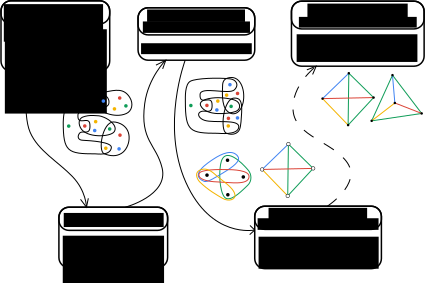
\includegraphics{origen_problema.pdf}
  \end{figure}
\end{frame}

\begin{frame}
  \frametitle{Tamaño de un thrackle de triángulos}
  \begin{block}{}
    Atacamos el problema buscando cotas superiores e inferiores del tamaño
    máximo de un thrackle de triángulos.
  \end{block}
  \begin{figure}[htb]
    \centering
    \input{cotas.pdf_tex}
  \end{figure}
\end{frame}

\begin{frame}
  \frametitle{¿Qué se sabe hasta ahora?, cota inferior}
  Cualquier conjunto de $n$ puntos tiene al menos $\lfloor\frac{n^2}{12}\rfloor$ triángulos
  disjuntos en aristas que contienen al mismo punto en su interior

  [J. Cano, L. Barba, T. Sakai and J. Urrutia].
  \begin{figure}[htb]
    \def\svgwidth{3cm}
    \input{triangulos_punto_interior.pdf_tex}
  \end{figure}
  \begin{itemize}[leftmargin=2cm]
    \item[$\implies$] Para todo conjunto de $n$ puntos en posición convexa, siempre existe un
      thrackle con $\lfloor\frac{n^2}{12}\rfloor$ triángulos.
  \end{itemize}
  Si $3|n$ entonces existe un thrackle con $\frac{n^2}{9}+1$ triángulos.
  \begin{itemize}[leftmargin=1cm]
    \item ¿Se cumple para todo $n$?
  \end{itemize}
\end{frame}

\begin{frame}
  \frametitle{¿Qué se sabe hasta ahora?, cota superior}
  Caracterización de los segmentos restantes en un conjunto de triángulos
  disjuntos en aristas de tamaño máximo [H. Hanani, 1975].
  \begin{figure}[htb]
    \scriptsize
    \input{hanani.pdf_tex}
  \end{figure}
  Un thrackle puede tener máximo $\frac{n^2}{6}-O(n)$ triángulos.
\end{frame}

\begin{frame}[c]
  \begin{center}
    \Huge Resultados: Puntos en posición general.
  \end{center}
\end{frame}

\begin{frame}
  \frametitle{Posición general, $3\le n\le 7$}
  \begin{columns}
      \hspace{0.1cm}
    \begin{column}{0.45\textwidth}
      \begin{teo}
        El tamaño máximo de un thrackle $T_n$ en un conjunto de $n$
        puntos para $3\le n\le 7$ es:

        \vspace{0.5cm}
        \centering
        \begin{tabular}{| c | c |}
          \hline
          \textbf{$n$} & \textbf{$T_n$} \\ \hline
          3 & 1 \\ \hline 
          4 & 1 \\ \hline
          5 & 2 \\ \hline
          6 & 4 \\ \hline
          7 & 7 \\ \hline
        \end{tabular}
        \vspace{0.5cm}
      \end{teo}
    \end{column}
    \hfill
    \begin{column}{0.5\textwidth}
      \begin{center}
      \begin{figure}[htb]
        \centering
        \input{n_5_pos_general.pdf_tex}
      \end{figure}
      \end{center}
    \end{column}
  \end{columns}
\end{frame}

\begin{frame}
  \frametitle{Posición general, $n=8$}
  Algoritmo de backtracking para determinar que el tamaño máximo de un thrackle
  sobre todo conjunto de 8 puntos.
  \begin{itemize}
    \item Por la cota superior debe haber a lo sumo 8 triángulos.
    \item La cota inferior más alta, ignorando que $3\nmid8$ es $\sim8$.
  \end{itemize}
  \vspace{0.3cm}
  El algoritmo busca un thrackle de 8 triángulos para cada conjunto de 8
  puntos.
\end{frame}

\begin{frame}
  \frametitle{Algoritmo de backtracking 1}
  \begin{figure}[htb]
    \includegraphics<1>{alg_1_1.pdf}
    \includegraphics<2>{alg_1_2.pdf}
    \includegraphics<3>{alg_1_3.pdf}
    \includegraphics<4>{alg_1_4.pdf}
    \includegraphics<5>{alg_1_5.pdf}
    \includegraphics<6>{alg_1_6.pdf}
    \includegraphics<7>{alg_1_7.pdf}
    \includegraphics<8>{alg_1_8.pdf}
    \includegraphics<9>{alg_1_9.pdf}
    \includegraphics<10>{alg_1_10.pdf}
    \includegraphics<11>{alg_1_11.pdf}
    \includegraphics<12>{alg_1_12.pdf}
    \includegraphics<13>{alg_1_13.pdf}
  \end{figure}
\end{frame}

\begin{frame}
  \frametitle{Orden de los triángulos}
  \begin{figure}[htb]
    \includegraphics<1>{orden_de_triangulos.pdf}
  \end{figure}
\end{frame}

\begin{frame}
  \frametitle{Resultados de la ejecución, para $n=8$}
  La ejecución del Algoritmo 1 para cada uno de los 3315 conjunto de puntos,
  utilizando un procesador Intel Core i7, arrojó los siguientes resultados:
  \begin{itemize}[leftmargin=1cm]
    \item Existe un thrackle de tamaño 8 para cada conjunto de 8 puntos.
    \item Nodos recorridos: $\sim$7,838.63 en promedio
    \item Tiempo: 1.34 segundos (0.404 ms en promedio)
  \end{itemize}

  \pause
  \vspace{0.5cm}
  \begin{teo}
    Todo thrackle sobre cualquier conjunto de 8 puntos tiene máximo 8~triángulos.
  \end{teo}
\end{frame}

\begin{frame}
  \frametitle{Árbol de búsqueda, para $n=8$}
  \begin{figure}[htb]
    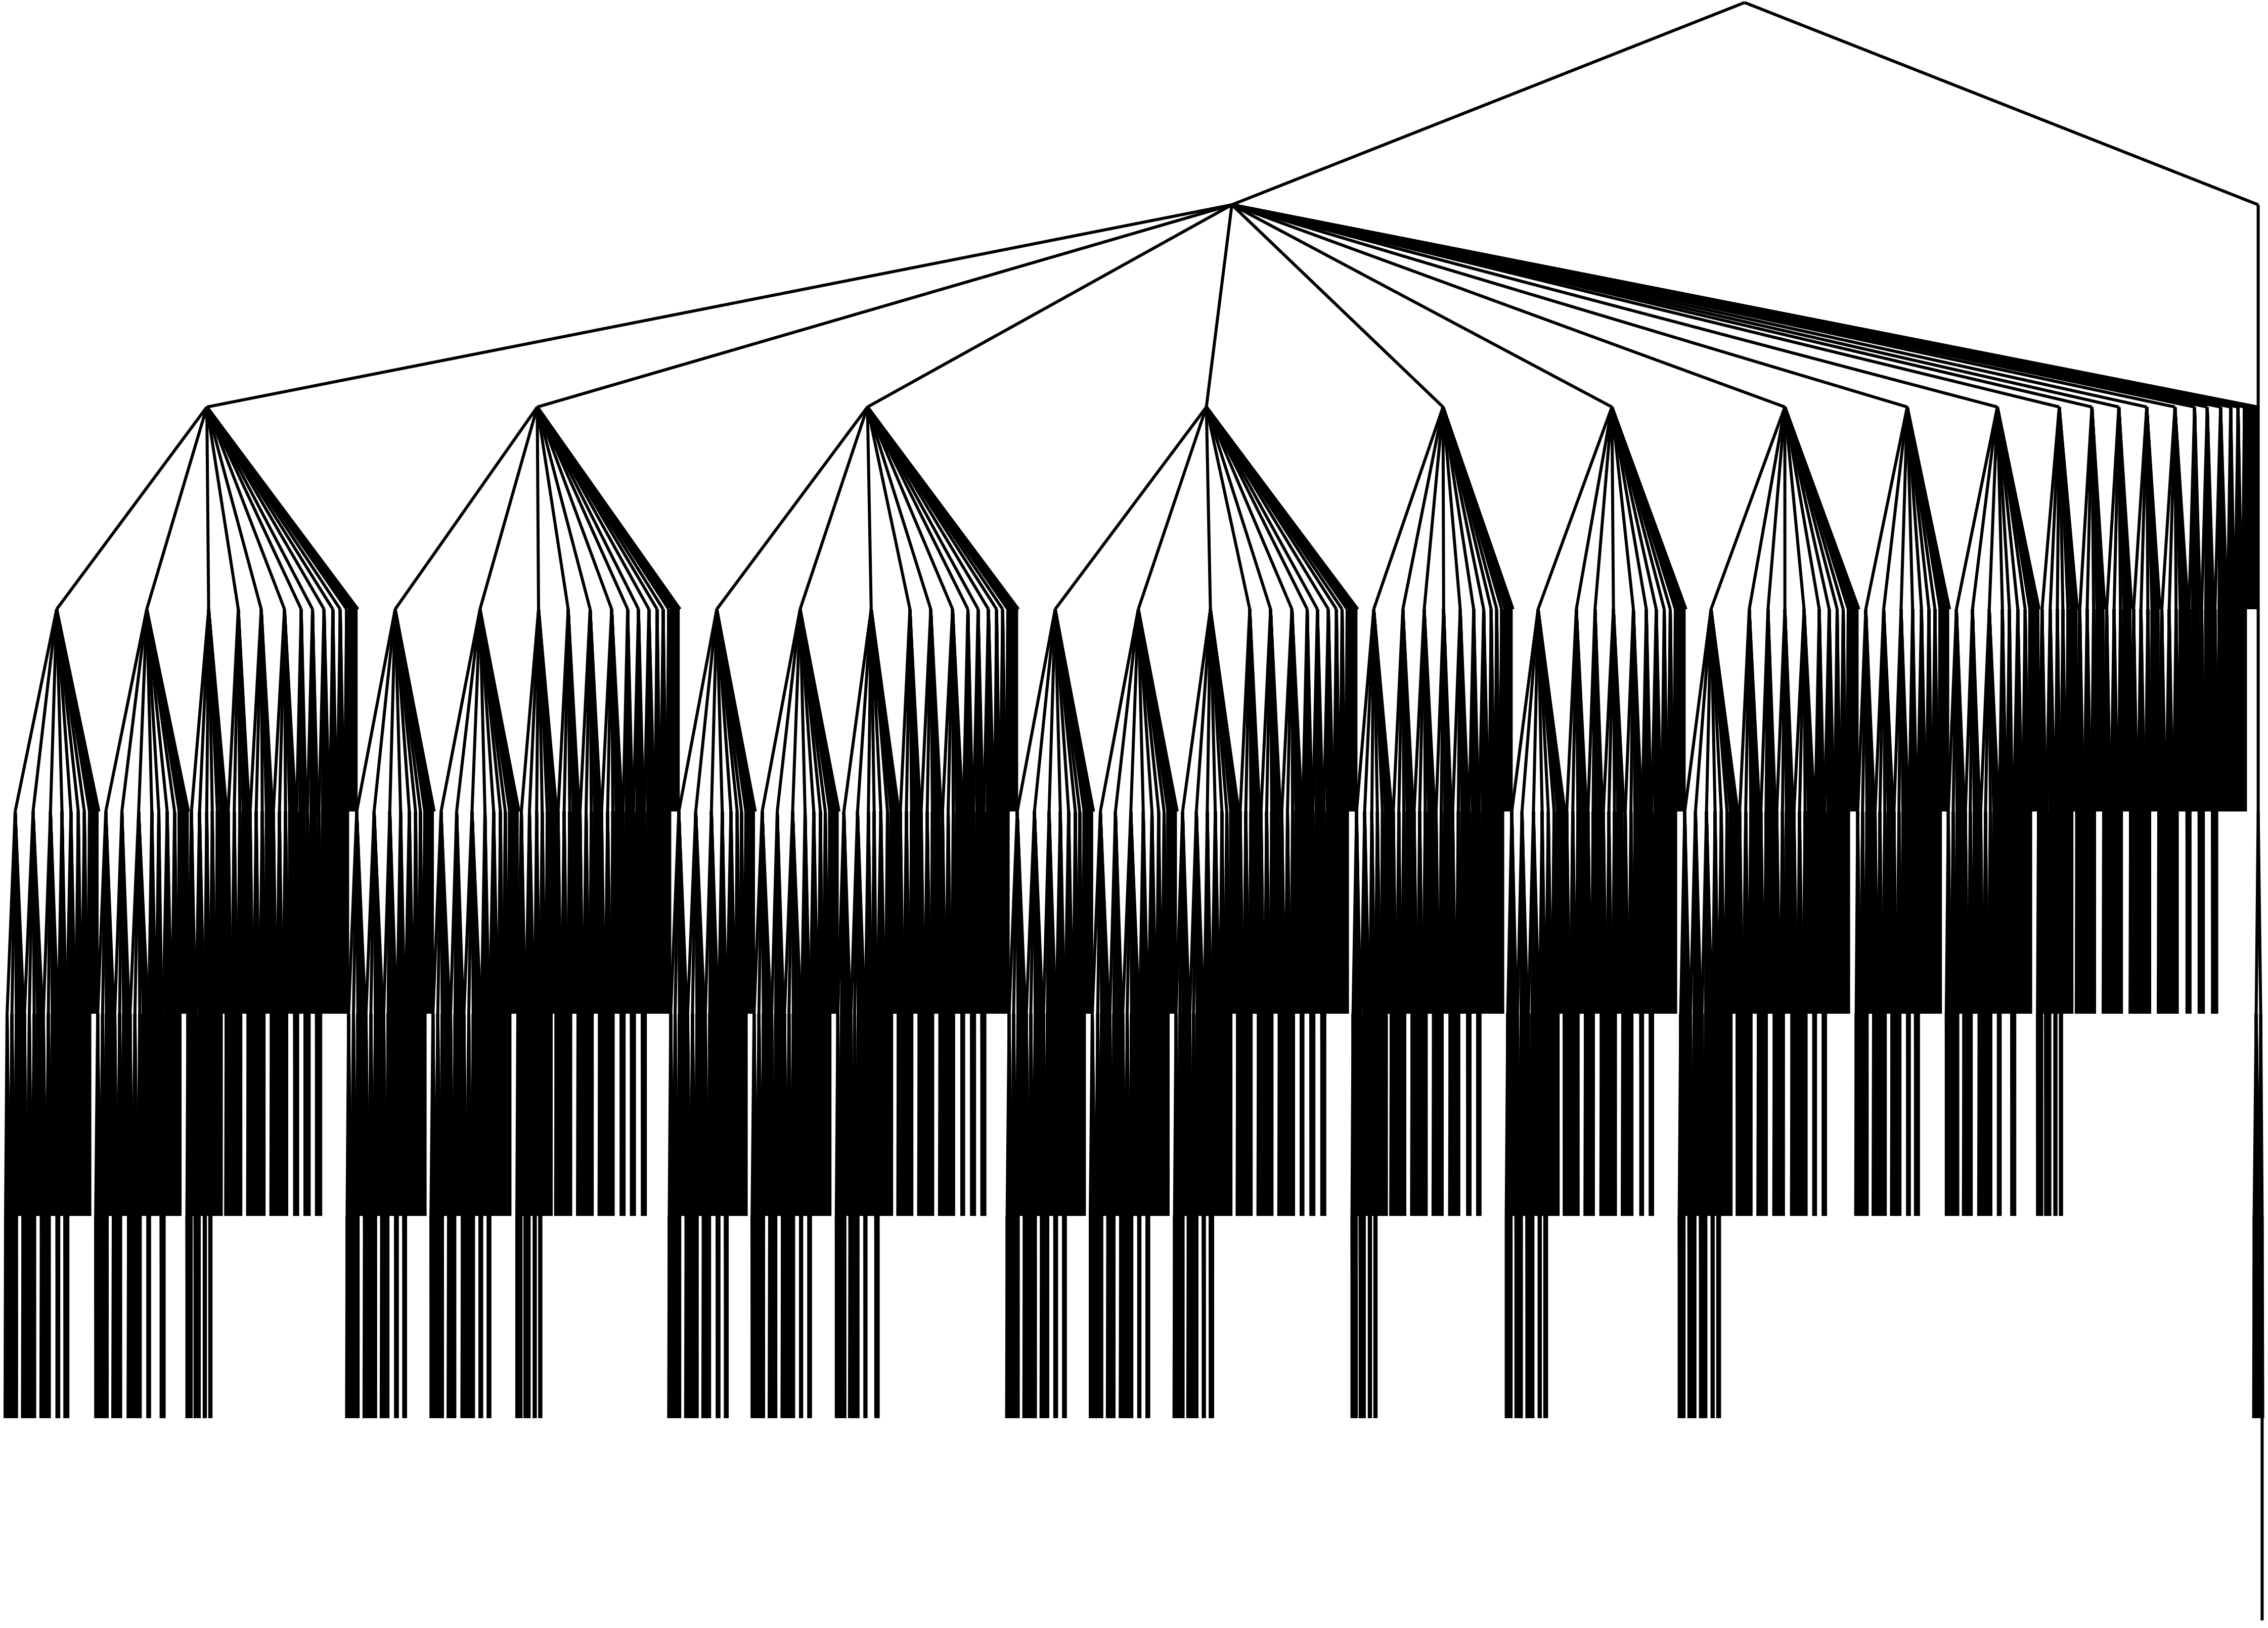
\includegraphics[width=0.9\textwidth]{n_8_thr_first.png}
  \end{figure}
\end{frame}

\begin{frame}
  \frametitle{Posición general, $n=9$}
  El tamaño máximo de un thrackle debe estar en el intervalo $[9,12]$.
  \vspace{0.3cm}

  Algoritmo 2 es un versión modificada del anterior que explora el árbol
  completamente y almacena el tamaño máximo de los thrackles.
  \vspace{0.3cm}

  La ejecución sobre los 158,817 conjuntos de puntos, tuvo las siguientes
  características:
  \begin{itemize}[leftmargin=1cm]
    \item Tiempo: $\sim9$ horas 57 minutos (225.5 ms en promedio)
    \item Nodos: $\sim$2,526,172.5 nodos en promedio
    \item Memoria: Máximo $148.8$ MB por conjunto de puntos
  \end{itemize}

  \vspace{0.3cm}
  \pause
  \begin{teo}
    Todo thrackle sobre cualquier conjunto de 9 puntos tiene máximo
    10~triángulos.
  \end{teo}
\end{frame}

\begin{frame}
  \frametitle{Árbol de búsqueda, para $n=9$}
  \begin{figure}[htb]
    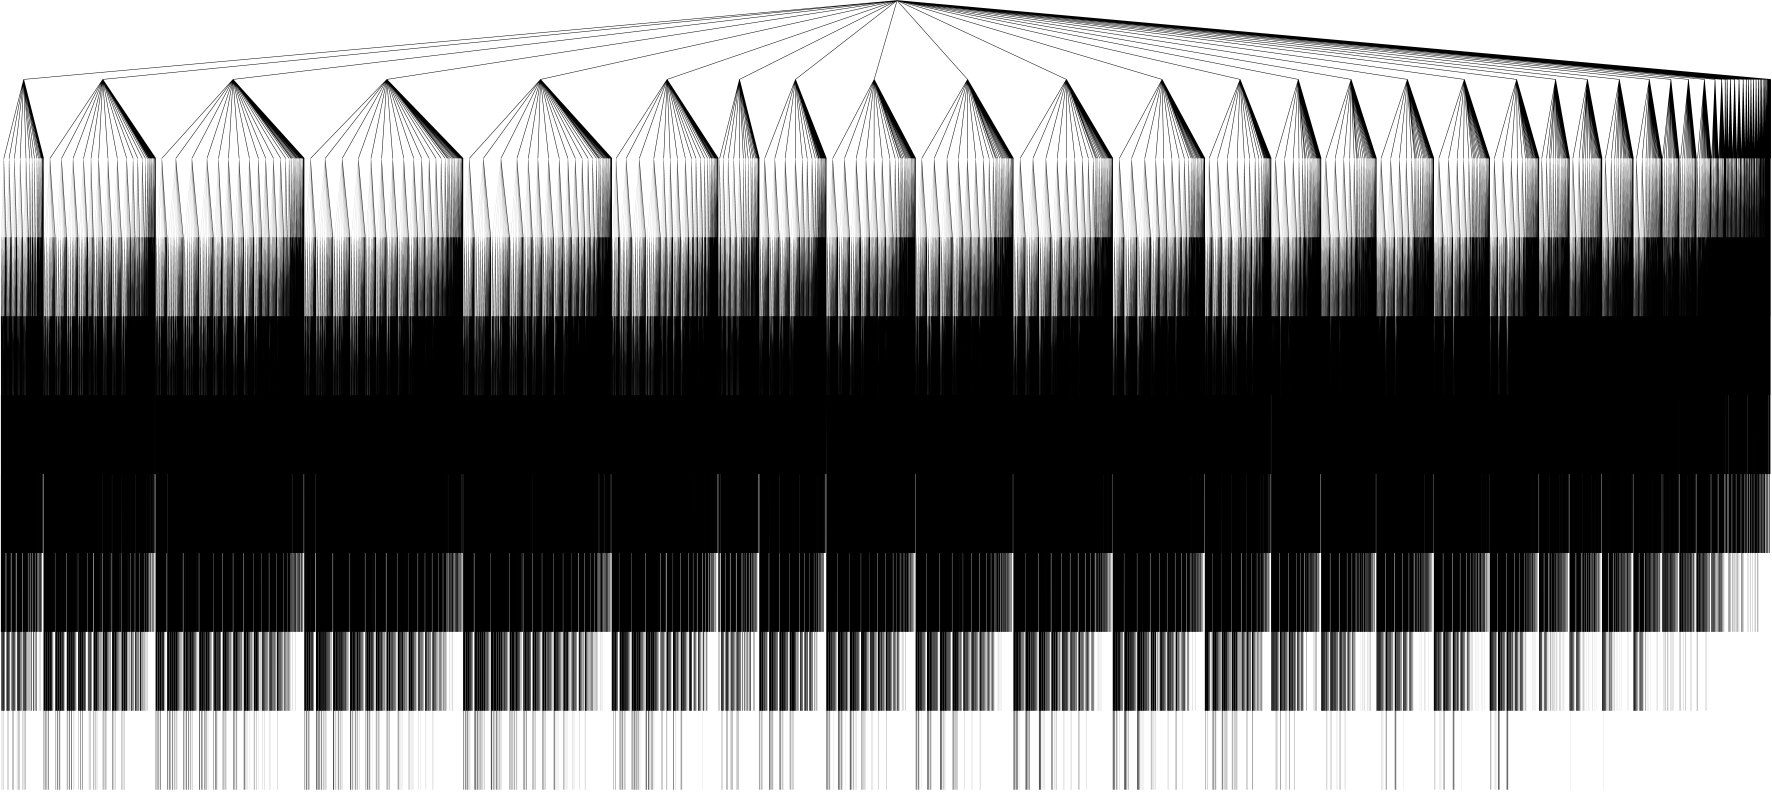
\includegraphics[width=\textwidth]{n_9_thr_full.png}
  \end{figure}
\end{frame}

\begin{frame}
  \frametitle{Posición general, $n=10$}
  El tiempo de ejecución del Algoritmo 2 se hace muy grande. El árbol de
  búsqueda para posición convexa tiene las siguientes propiedades:
  \begin{itemize}
    \item Nodos: 305,532,771 nodos
    \item Tiempo: 12.86 segundos
    \item Memoria: 8.87 GB
      \begin{itemize}[leftmargin=1.5cm]
        \item[$\implies$] 5.84 años para explorar los 14,309,547 conjuntos de puntos.
      \end{itemize}
  \end{itemize}
  \begin{overprint}
    \onslide<1>
    Con varias ejecuciones del Algoritmo 1 se obtuvo que:
    \begin{itemize}
      \item Todo conjunto de 10 puntos tiene un thrackle con 11 triángulos.
        \begin{itemize}[leftmargin=1cm]
          \item (Ejecución de 35 minutos).
        \end{itemize}
      \item Aproximadamente 79,712 conjuntos de 10 puntos (0.56\%) no tienen un
        thrackle con 12 triángulos.
        \begin{itemize}[leftmargin=1cm]
          \item (Ejecución de 30 horas).
        \end{itemize}
    \end{itemize}
    \onslide<2>
    \begin{teo}
      Todo conjunto de 10 puntos tiene un thrackle de tamaño 11.
    \end{teo}
    \vspace{0.5cm}
    \begin{teo}
      Hay thrackles cuyo tamaño máximo es 11.
    \end{teo}
  \end{overprint}
\end{frame}

\begin{frame}
  \frametitle{¿Cuánto tarda el Algoritmo 2?}
  \begin{overprint}
    \onslide<1>
    \begin{itemize}
      \item El número de iteraciones es al menos igual al número de thrackles
        distintos.
      \item El peor caso ocurre para el conjunto de puntos con mayor número de
        thrackles distintos.
    \end{itemize}
    \onslide<2>
    \begin{conj}
      Los conjuntos de puntos con mayor número de thrackles son 2-convexos
    \end{conj}
  \end{overprint}
  \vspace{0.2cm}
  \begin{figure}[htb]
    \centering
    \def\svgwidth{10cm}
    \input{2-convex_n_8.pdf_tex}
  \end{figure}
\end{frame}

\begin{frame}[c]
  \begin{center}
    \Huge Resultados: Puntos en posición convexa.
  \end{center}
\end{frame}

\begin{frame}[t]
  \frametitle{Construcción para todo $n$}
  Se extendió la cota inferior del tamaño de un thrackle, para incluir los
  casos en que $3\nmid n$.

  \begin{columns}
    \begin{column}{0.4\textwidth}
      \centering
      \begin{figure}
        \def\svgwidth{5cm}
        \only<1>{\input{3_n_1.pdf_tex}}
        \only<2>{\input{3_n_2.pdf_tex}}
        \only<3>{\input{3_n_3.pdf_tex}}
        \only<4>{\input{3_n_4.pdf_tex}}
        \only<5>{\input{3_n_5.pdf_tex}}
        \only<6>{\input{3_n_6.pdf_tex}}
        \only<7>{\input{3_n_7.pdf_tex}}
        \only<8>{\input{3_n_8.pdf_tex}}
        \only<9>{\input{3_n_9.pdf_tex}}
        Caso $3|n$.
      \end{figure}
    \end{column}
    \begin{column}{0.5\textwidth}
      \begin{teo}
        Todo conjunto de $n$ puntos en el plano en posición convexa, con $n\ge6$,
        tiene un thrackle de triángulos, cuyo tamaño $k(n)$ es: 
        \[
          k(n) = 
          \begin{cases}
            \frac{n^2}{9}+1 &\ \text{si}\ 3|n \\
            \frac{n^2}{9}-\frac{n}{18}+\frac{35}{18} &\ \text{si}\ 6|n-1 \\
            \frac{n^2}{9}-\frac{n}{18}+\frac{13}{9}  &\ \text{si}\ 6|n-4 \\
            \frac{n^2}{9}-\frac{n}{9}+\frac{7}{9}   &\ \text{si}\ 6|n-5 \\
            \frac{n^2}{9}-\frac{n}{9}+\frac{16}{9}   &\ \text{si}\ 6|n-2
          \end{cases}
        \]
      \end{teo}
    \end{column}
  \end{columns}
\end{frame}

\begin{frame}
  \frametitle{Número de 1-factorizaciones de $K_{n,n}$}
  \centering
  \begin{figure}
    \def\svgwidth{10cm}
    \input{T.pdf_tex}
  \end{figure}
\end{frame}

\begin{frame}
  \frametitle{Número mínimo de thrackles}
  Determinamos cuántos thrackles distintos tiene un conjunto de $n$ puntos en
  posición convexa.

  Encontramos una cota inferior analítica para este valor cuando $6|n$.\\
  \begin{columns}
    \begin{column}{0.3\textwidth}
      \begin{center}
        \begin{tabular}{| l | c |}
          \hline
          \textbf{n} & \textbf{Thrackles} \\ \hline
          3 & 1 \\ \hline 
          4 & 4 \\ \hline
          5 & 15 \\ \hline
          6 & 30 \\ \hline
          7 & 30 \\ \hline
          8 & 120 \\ \hline
          9 & 3156 \\ \hline
          10 & 47460 \\ \hline
        \end{tabular}
      \end{center}
    \end{column}
    \begin{column}{0.7\textwidth}
      \begin{teo}
        Hay al menos
        $$(p(n/3)-p(n/3-1))\frac{(\frac{n}{3})!\cdot6^{\frac{n}{3}-2}\cdot2^{\frac{n}{6}-1}}{(\frac{n}{6})!\binom{n/3}{2}}$$
        thrackles de triángulos distintos, para $n$ puntos en posición
        convexa con $6|n$. Donde $p(n)$ es el número de formas de sumar $n$
        (función de partición).
      \end{teo}
    \end{column}
  \end{columns}
\end{frame}

\begin{frame}
  \frametitle{Orden de triángulos en posición convexa}
  El Algoritmo 1 tiene mejor tiempo de ejecución si ordenamos los triángulos.
  \begin{overprint}
    \onslide<1>
    \begin{figure}[htb]
      \centering
      \input{orden_triangulos.pdf_tex}
    \end{figure}
    \onslide<2>
    \begin{figure}[htb]
      \centering
      \input{orden_triangulos_1.pdf_tex}
    \end{figure}
    \onslide<3>
    \begin{figure}[htb]
      \centering
      \input{orden_triangulos_2.pdf_tex}
    \end{figure}
    \begin{itemize}
      \item Acelera búsquedas utilizando el Algoritmo 1.
      \item ¿Puede generalizarse a conjuntos de puntos en posición general?
    \end{itemize}
  \end{overprint}
\end{frame}

\begin{frame}
  \frametitle{Conclusiones}
  \begin{itemize}
    \item Encontramos evidencia para creer que el tamaño máximo de un thrackle
      de triángulos sobre un conjunto de $n$ puntos es a lo sumo el valor
      conjeturado de $\frac{n^2}{9}+2$.
      \begin{itemize}
          \item La conjetura es cierta para $3\le n\le 9$.
          \item No encontramos un contraejemplo, pero la cota inferior se acerca
            al valor conjeturado.
      \end{itemize}
    \item La complejidad computacional de una búsqueda exhaustiva crece bastante
      rápido.
      \begin{itemize}
          \item Para $n=10$ se podría realizar una búsqueda utilizando
            paralelización y más recursos computacionales.
          \item Para posición convexa obtuvimos una cota inferior para todo
            $n$, pero todavía es menor al calculado computacionalmente.
      \end{itemize}
  \end{itemize}
\end{frame}

\begin{frame}
  \frametitle{Trabajo futuro}
  Caracterización del resto de un thrackle de triángulos.
  \begin{figure}
    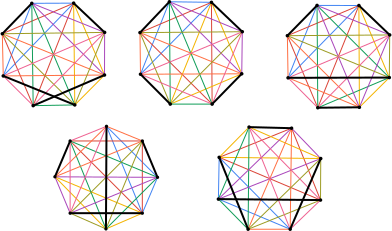
\includegraphics{resto_thrackles.pdf}
  \end{figure}
\end{frame}

\begin{frame}
  \frametitle{Trabajo futuro}
  \begin{itemize}
    \item Los conjuntos de 8 y 9 puntos con mayor número de thrackles maximales
      distintos conjuntos de puntos 2-convexos.
      \begin{itemize}
        \item ¿Es esto cierto para todo $n$?
      \end{itemize}
      \vspace{0.5cm}
    \item El orden de los triángulos en posición convexa reduce
      significativamente el tiempo de ejecución.
      \begin{itemize}
        \item ¿Se puede generalizar esta idea a posición general?
        \item ¿Se puede modificar el Algoritmo 2 para tomar ventajas de esta generalización?
      \end{itemize}
  \end{itemize}
\end{frame}

\begin{frame}
  \frametitle{Código fuente}
  \begin{figure}[htb]
    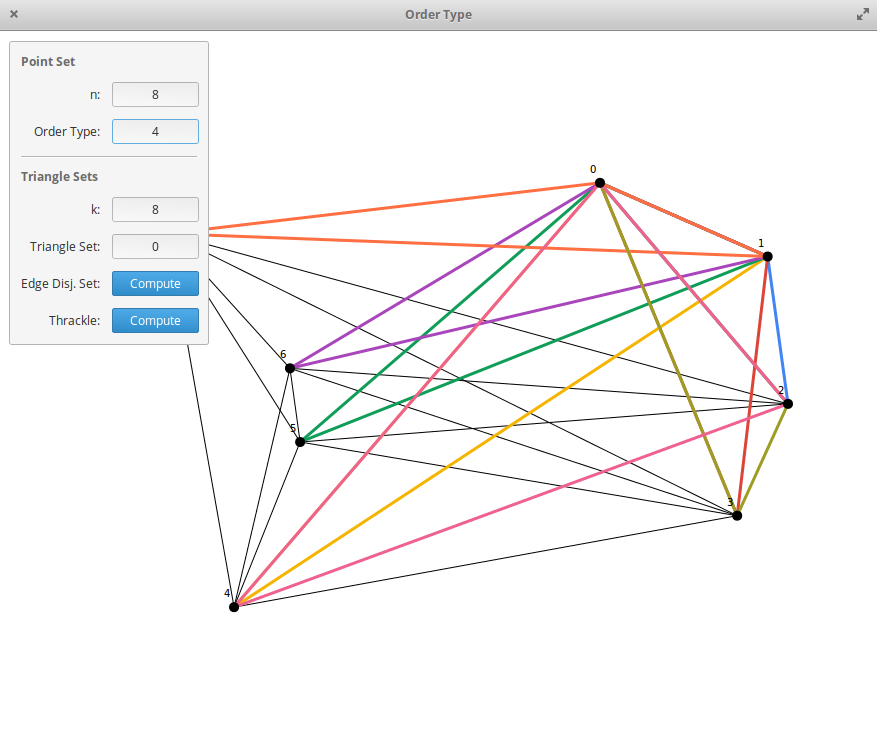
\includegraphics[width=0.7\textwidth]{aplicacion.png}

    \url{http://github.com/cinvestavcs-mexicocity/Triangle-thrackles}
  \end{figure}
\end{frame}

\begin{frame}[c]
  \begin{center}
    \Huge ¡Gracias!
  \end{center}
\end{frame}

\end{document}
